\documentclass[10pt]{exam}

\usepackage[utf8]{inputenc}
\usepackage{verbatim, multicol, tabularx, graphicx, float, xcolor, colortbl}
\usepackage{amsmath,amsthm, amssymb, latexsym, listings, qtree}

\lstset{frame=tb,
  language=Java,
  aboveskip=1mm,
  belowskip=0mm,
  showstringspaces=false,
  columns=flexible,
  basicstyle={\ttfamily},
  numbers=none,
  frame=single,
  breaklines=true,
  breakatwhitespace=true
}

\textwidth = 6.5 in
\textheight = 9 in
\oddsidemargin = 0.0 in
\evensidemargin = 0.0 in
\topmargin = -0.25 in
\headheight = 0.0 in
\headsep = 0.0 in
\parskip = 0.0in
\parindent = 0.0in

\def\ojoin{\setbox0=\hbox{$\bowtie$}%
  \rule[-.02ex]{.25em}{.4pt}\llap{\rule[\ht0]{.25em}{.4pt}}}
\def\leftouterjoin{\mathbin{\ojoin\mkern-5.8mu\bowtie}}
\def\rightouterjoin{\mathbin{\bowtie\mkern-5.8mu\ojoin}}
\def\fullouterjoin{\mathbin{\ojoin\mkern-5.8mu\bowtie\mkern-5.8mu\ojoin}}

\def\a{& $\blacksquare\blacksquare\blacksquare$ & [ B ] & [ C ] & [ D ] \\}
\def\b{& [ A ] & $\blacksquare\blacksquare\blacksquare$ & [ C ] & [ D ] \\}
\def\c{& [ A ] & [ B ] & $\blacksquare\blacksquare\blacksquare$ & [ D ] \\}
\def\d{& [ A ] & [ B ] & [ C ] & $\blacksquare\blacksquare\blacksquare$ \\}



\title{CS 4400 Exam 3 Practice}
\date{ER-Relational Mapping, SQL, Relational Design}
\setcounter{page}{1}
\begin{document}

\maketitle
\thispagestyle{empty}
\firstpageheader{}               {\tiny Copyright \textcopyright\ 2016 All rights reserved. Duplication and/or usage for purposes of any kind without permission is strictly forbidden.}
                {}


\runningheader{}
{\small Name: \underline{\hspace{2.8in}} GTAccount: \underline{\hspace{1.4in}} Section: \underline{\hspace{.5in}}}
{}

%% \footer{Page \thepage\ of \numpages}
%%               {}
%%               {Points available: \pointsonpage{\thepage} -
%%                points lost: \makebox[.5in]{\hrulefill} =
%%                points earned:  \makebox[.5in]{\hrulefill}.
%%               Graded by: \makebox[.5in]{\hrulefill}}


\ifprintanswers
\begin{center}
{\LARGE ANSWER KEY}
\end{center}
\vspace{.25in}
\else
\vspace{0.1in}
\hbox to \textwidth{Name: \enspace\hrulefill}
\vspace{0.2in}
\hbox to \textwidth{GT account (gtg, gth, msmith3, etc): \underline{\hspace{2in}} Section (e.g., B1): \underline{\hspace{.75in}}}
\vspace{0.2in}
\hbox to \textwidth{Signature: \enspace\hrulefill}

\vfill

\begin{itemize}
\item Failure to properly fill in the information on this page will result in a deduction of up to 4 points from your exam score.
\item Signing signifies that you agree to comply with the {\bf Academic Honor Code of Georgia Tech}.
\item Calculators and cell phones are NOT allowed.
\end{itemize}

\fi


% Points Table
%\begin{center}
%\addpoints
%\gradetable[v][pages]
%\end{center}

Completely fill in the box corresponding to your answer choice for each question.

\ifprintanswers
\begin{tabular}{lcccc}\\
  1. \c
  2. \c
  3. \c
  4. \a
  5. \d
  6. \c
  7. \b
  8. \a
  9. \b
  10. \c
  11. \d
  12. \c
  13. \d
  14. \a
  15. \a
  16. \b
  17. \d
  18. \d
  19. \a
  20. \b
\end{tabular}
\else
\begin{tabular}{lcccc}\\
  1. & [ A ] & [ B ] & [ C ] & [ D ] \\
  2. & [ A ] & [ B ] & [ C ] & [ D ] \\
  3. & [ A ] & [ B ] & [ C ] & [ D ] \\
  4. & [ A ] & [ B ] & [ C ] & [ D ] \\
  5. & [ A ] & [ B ] & [ C ] & [ D ] \\
  6. & [ A ] & [ B ] & [ C ] & [ D ] \\
  7. & [ A ] & [ B ] & [ C ] & [ D ] \\
  8. & [ A ] & [ B ] & [ C ] & [ D ] \\
  9. & [ A ] & [ B ] & [ C ] & [ D ] \\
  10. & [ A ] & [ B ] & [ C ] & [ D ] \\
  11. & [ A ] & [ B ] & [ C ] & [ D ] \\
  12. & [ A ] & [ B ] & [ C ] & [ D ] \\
  13. & [ A ] & [ B ] & [ C ] & [ D ] \\
  14. & [ A ] & [ B ] & [ C ] & [ D ] \\
  15. & [ A ] & [ B ] & [ C ] & [ D ] \\
  16. & [ A ] & [ B ] & [ C ] & [ D ] \\
  17. & [ A ] & [ B ] & [ C ] & [ D ] \\
  18. & [ A ] & [ B ] & [ C ] & [ D ] \\
  19. & [ A ] & [ B ] & [ C ] & [ D ] \\
  20. & [ A ] & [ B ] & [ C ] & [ D ] \\
\end{tabular}

\fi

\vspace{.5in}

Number missed: \makebox[.5in]{\hrulefill} Written Score: \makebox[.5in]{\hrulefill}\\\\
+ Queries score: \makebox[.5in]{\hrulefill} = Final Score: \makebox[.5in]{\hrulefill}

\newpage

\newpage

\pointsinmargin
\bracketedpoints

\marginpointname{}

Refer to the following EER diagram for Questions 1 -- 7

\begin{center}
  \hspace{-.5in}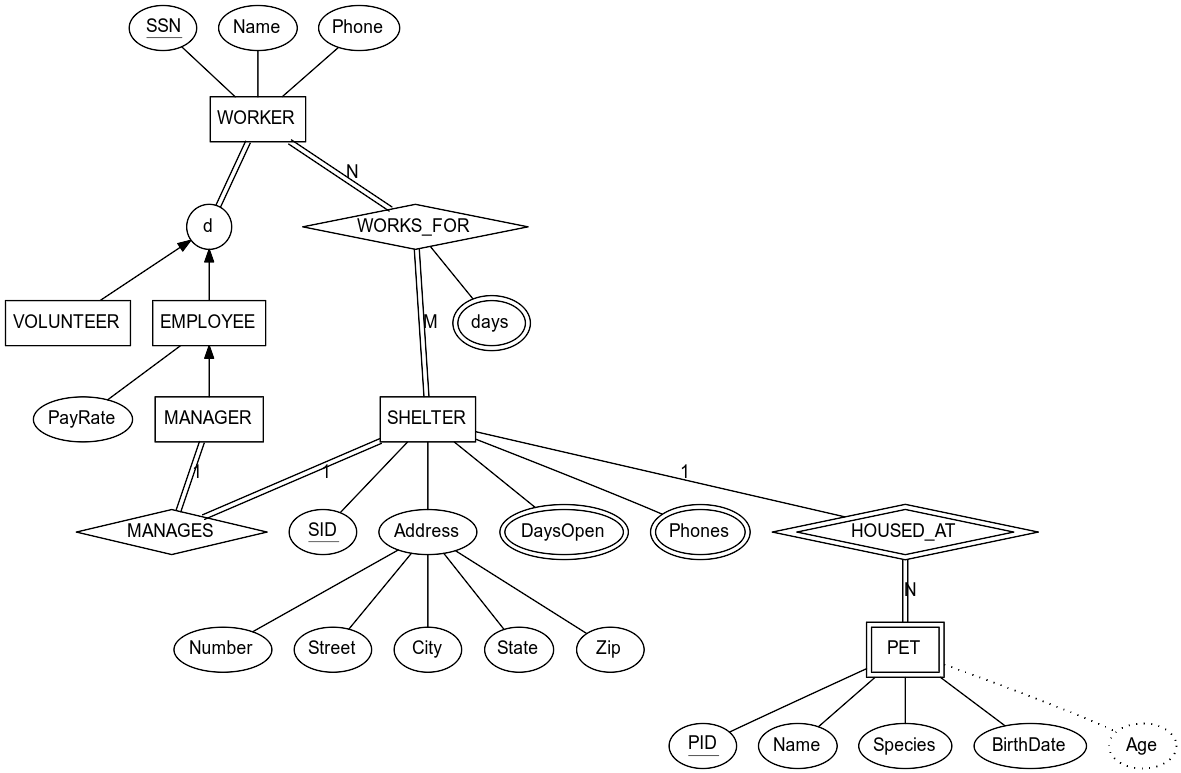
\includegraphics[width=7in]{humane-society.png}
\end{center}

\newpage

\begin{questions}

\question[4] Which of the following (sets of) relation schemas is a correct mapping of the SHELTER entity type? (Disregard the MANAGES relationship.)

\begin{choices}
\choice SHELTER(\underline{SID}, Number, Street, City, State, Zip, DaysOpen, Phones)
\choice SHELTER(\underline{SID}, Number, Street, City, State, Zip, Phones), DaysOpen(\underline{SID, Day})
\correctchoice SHELTER(\underline{SID}, Number, Street, City, State, Zip), DaysOpen(\underline{SID, Day}), Phones(\underline{SID, Phone})
\choice All of the above.
\end{choices}

\question[4] Which of the following relation schemas is a correct mapping of the PET entity type?

\begin{choices}
\choice PET(\underline{PID}, Name, Species, BirthDate, Age)
\choice PET(\underline{PID}, Name, Species, BirthDate)
\correctchoice PET(\underline{PID, SID}, Name, Species, BirthDate)
\choice None of the above
\end{choices}

\question[4] Which of the following sets of relation schemas is a correct mapping of the WORKS\_FOR relationship (Disregard multivalued attributes of SHELTER.)?

\begin{choices}
\choice WORKER(\underline{SSN}, Name, Phone, SID), SHELTER(\underline{SID}, Number, Street, City, State, Zip)
\choice WORKER(\underline{SSN}, Name, Phone), SHELTER(\underline{SID}, Number, Street, City, State, Zip, SSN)
\correctchoice WORKER\_SHELTER(\underline{SSN, SID}), WORK\_DAYS(\underline{SSN, SID, Day})
\choice WORKER\_SHELTER(\underline{SSN, SID}, Days)
\end{choices}

\question[4] What's the least number of tables necessary to model the WORKER - VOLUNTEER - EMPLOYEE - MANAGER class hierarchy?

\begin{choices}
\correctchoice 1
\choice 2
\choice 3
\choice 4
\end{choices}

\question[4] Which of the following sets of relation schemas acceptably represenents the WORKER - VOLUNTEER - EMPLOYEE - MANAGER class hierarchy?

\begin{choices}
\choice WORKER(SSN, Name, Phone), VOLUNTEER(SSN), EMPLOYEE(SSN,PayRate), MANAGER(SSN)
\choice EMPLOYEE(SSN, Name, Phone, PayRate, IsManager), VOLUNTEER(SSN)
\choice WORKER(SSN, Name, Phone, PayRate, IsManager)
\correctchoice All of the above.
\end{choices}


\question[4] Which of the following create table statements creates a PET table that accurately models the PET entity type?

\begin{choices}
\choice create table pet(PID int primary key, Name varchar(20), Species varchar(20), Birthdate date)
\choice create table pet(PID int primary key, Name varchar(20), Species varchar(20), Birthdate date, SID int)
\correctchoice create table pet(PID int, Name varchar(20), Species varchar(20), Birthdate date, SID int, primary key (PID, SID), foreign key (SID) references shelter(SID))
\choice None of the above.
\end{choices}

\question[4] Which of the following create table statements creates a table that accurately models the WORKS\_FOR relationship? (Disregard multivalued attributes.)

\begin{choices}
\choice create table worker\_shelter(SSN int, SID int, days enum (M, Tu, W, Th, F))
\correctchoice create table worker\_shelter(SSN int, SID int, primary key (SSN, SID), foreign key (SSN) references worker (SSN), foreign key (SID) references shelter (SID))
\choice create table worker\_shelter(SSN int, SID int, primary key (SSN))
\choice None of the above.
\end{choices}

\newpage

Refer to the following create table statements and table data for Questions 8 -- 10.

\begin{lstlisting}[language=sql]
create table dorm (
    dorm_id integer primary key auto_increment,
    name text not null,
    spaces integer
);


create table student (
    student_id integer primary key auto_increment,
    name text,
    gpa float(3,2),
    dorm_id integer not null,
    foreign key (dorm_id) references dorm(dorm_id)
);
\end{lstlisting}


\begin{verbatim}
mysql> select * from dorm;
+---------+-----------+--------+
| dorm_id | name      | spaces |
+---------+-----------+--------+
|       1 | Armstrong |    124 |
|       2 | Brown     |    158 |
+---------+-----------+--------+
2 rows in set (0.00 sec)

mysql> select * from student;
+------------+-------+------+---------+
| student_id | name  | gpa  | dorm_id |
+------------+-------+------+---------+
|          1 | Alice | 3.60 |       1 |
|          2 | Bob   | 2.70 |       1 |
+------------+-------+------+---------+
2 rows in set (0.00 sec)

\end{verbatim}

\question[4] Which of the following insert statements will succeed?

\begin{choices}
\correctchoice {\tt insert into dorm (name, spaces) values('Caldwell', 158);}
\choice {\tt insert into dorm values('Caldwell', 158);}
\choice {\tt insert into dorm (name, spaces) values(null, 158);}
\choice All of the above.
\end{choices}

\question[4] Which of the following insert statement is certain to succeed?

\begin{choices}
\choice {\tt insert into student (name, gpa, dorm\_id) values ('Cheng', 3.6, 3);}
\correctchoice {\tt insert into student (name, gpa, dorm\_id) values ('Cheng', 3.6, 1);}
\choice {\tt insert into student (name, gpa) values ('Cheng', 3.6);}
\choice All of the above.
\end{choices}

\question[4] Which of the following delete statements will fail?

\begin{choices}
\choice {\tt delete from student}
\choice {\tt delete from dorm where name = 'Brown';}
\correctchoice {\tt delete from dorm where name = 'Armstrong';}
\choice None of the above.
\end{choices}

\newpage

For questions 11 -- 20 use this relation schema and set of functional dependencies $F$:\\

$ATL-TRANSIT(DriverSsn, EmpName, RouteNum, BusId, RouteDate, ServiceDate)$
\begin{eqnarray*}
  DriverSsn & \rightarrow & RouteNum\\
  RouteNum,RouteDate & \rightarrow & BusId\\
  BusId & \rightarrow & ServiceDate\\
  RouteNum,RouteDate & \rightarrow & DriverSsn\\
  DriverSsn & \rightarrow & EmpName
\end{eqnarray*}

\question[4] Which one of the following functional dependencies is in $F^+$?

\begin{choices}
\choice $RouteDate \rightarrow  BusId$
\choice $ServiceDate \rightarrow BusId$
\choice $RouteNum \rightarrow BusId$
\correctchoice $BusId,DriverSsn,EmpName \rightarrow BusId$
\end{choices}

\question[4] What is $\{RouteNum,RouteDate\}^+$ with respect to $F$?

\begin{choices}
\choice $\{RouteNum, RouteDate\}$
\choice $\{RouteNum, RouteDate, BusId, DriverSsn\}$
\correctchoice $\{RouteNum, RouteDate, BusId, DriverSsn, EmpName, ServiceDate\}$
\choice the empty set
\end{choices}

\question[4] Which of the following is a key for the ATL-TRANSIT schema?

\begin{choices}
\choice $DriverSsn$
\choice $\{RouteNum,RouteDate\}$
\choice $\{DriverSsn,RouteDate\}$
\correctchoice Both B and C
\end{choices}

\question[4] What is the highest normal form that the ATL-TRANSIT schema satisfies?

\begin{choices}
\correctchoice 1NF
\choice 2NF
\choice 3NF
\choice BCNF
\end{choices}


\question[4] Suppose we decompose the ATL-TRANSIT schema into

$ATL1(DriverSsn, RouteNum, BusId, RouteDate, ServiceDate)$\\
$ATL2(DriverSsn, EmpName)$

Does that decomposition have the lossless join property?

\begin{choices}
  \correctchoice Yes
  \choice No
\end{choices}

\question[4] Suppose we decompose the ATL-TRANSIT schema into

$ATL1 (RouteNum, RouteDate, BusId)$\\
$ATL2 (DriverSsn, RouteNum, EmpName, ServiceDate)$

Does that decomposition have the lossless join property?

\begin{choices}
  \choice Yes
  \correctchoice No
\end{choices}

\newpage

For questions 11 -- 20 use this relation schema and set of functional dependencies $F$:\\

$ATL-TRANSIT(DriverSsn, EmpName, RouteNum, BusId, RouteDate, ServiceDate)$
\begin{eqnarray*}
  DriverSsn & \rightarrow & RouteNum\\
  RouteNum,RouteDate & \rightarrow & BusId\\
  BusId & \rightarrow & ServiceDate\\
  RouteNum,RouteDate & \rightarrow & DriverSsn\\
  DriverSsn & \rightarrow & EmpName
\end{eqnarray*}


\question[4] Which attribute is fully functionally dependent on the set of attributes $\{RouteNum, RouteDate\}$?

\begin{choices}
\choice $BusId$
\choice $DriverSsn$
\choice $EmpName$
\correctchoice all of the above
\end{choices}

\question[4] Which of the following attributes are prime attributes?

\begin{choices}
\choice Only DriverSsn
\choice Only RouteNum
\choice RouteNum and RouteDate
\correctchoice DriverSsn, RouteNum and RouteDate
\end{choices}

\question[4] Suppose we decompose the ATL-TRANSIT schema into

$ATL1(RouteNum, RouteDate, BusId, DriverSsn)$\\
$ATL2(DriverSsn, RouteDate, EmpName, ServiceDate)$

Which of those schemas is in 3NF?

\begin{choices}
\correctchoice ATL1
\choice ATL2
\choice Both ATL1 and ATL2
\choice None of the above
\end{choices}

\question[4] Consider the current state for our ATL-TRANSIT schema as shown below. What values could be inserted for the two missing column values, RouteNum and ServiceDate,  without violating any of the FDs that have been defined for the ATL-TRANSIT schema. The domain for RouteNum is $\{10, 11, 12, 13, 14\}$ and the domain for ServiceDate is any valid date

\begin{tabular}{|l|l|l|l|l|l|}\hline
{\bf DriverSsn} & {\bf EmpName} & {\bf RouteNum} & {\bf BusId} & {\bf RouteDate} & {\bf ServiceDate} \\\hline
111-22-3333 & Brown & 11 & 101 & 07-07-2007 & 06-06-2006 \\\hline
333-33-4444 & Smith & & 202 & 07-11-2007 & 07-12-2005 \\\hline
222-44-5555 & Green & 12 & 101 & 07-12-2007 & \\\hline
333-33-4444 & Smith & 10 & 203 & 07-12-2007 & 08-22-2006 \\\hline
\end{tabular}

\begin{choices}
\choice The values 11 for RouteNum and '07-12-2005' for ServiceDate
\correctchoice The values 10 for RouteNum and '06-06-2006' for ServiceDate
\choice The values 13 for RouteNum and '09-01-2006' for ServiceDate
\choice None of the above
\end{choices}

\end{questions}

\end{document}
